\chapter{Obserwacje i wyniki}
Przeprocesowanie dostarczonego zbioru danych zajęło 11 dni, co poskutkowało zebraniem około 30GB informacji na temat analizowanych domen.

\section{Typy odebranych odpowiedzi}
Wśród przeanalizowanych par domen i serwerów można zaobserwować kilka charakterystycznych typów odpowiedzi. Odpowiedzi mogą być dzielone na kategorie ze względu na różne kryteria. Pierwszym kryterium, które będzie brane pod uwagę w niniejszej pracy jest po prostu rozmiar pliku przechowującego informacje pobrane z serwera autorytatywnego. Jest to motywowane faktem, że w istocie im większy jest plik z odpowiedzią, tym spodziewamy się, że zawiera on więcej informacji na temat odpytywanej domeny. 

Pierwszym typem jest odpowiedź, która zajmowała na dysku specyficzną ilość miejsca -- 25123 bajty. Zaobserwowano, że uzyskano 626288 odpowiedzi tego typu. Rozmiar pliku jest swego rodzaju skutkiem ubocznym uproszczonej implementacji skanera. Trudno było przewidzieć wszystkie specyficzne przypadki towarzyszące transferowi strefy DNS. Zaobserwowana sytuacja jest właśnie jednym z tych nietypowych sytuacji i nawet program dig nie odzworowuje idealnie zachowania jakie powinno nastąpić w takiej sytuacji. przyczyna utworzenia opisanego wcześniej pliku nie jest jednoznacznie określona. Zostały podjęte próby ustalenia czym spowodowane jest takie zachowanie. W takich samych przypadkach program dig zwraca jedynie rekord DNS SOA i komunikat o błędzie (ang. \textit{communications error: end of file}). Zachowanie programu dig w dużym stopniu przypomina przekierowanie zapytania IXFR na AXFR (ang. \textit{AXFR fallback}) opisane między innymi w RFC1995\cite{RFC1995}. Wywołanie AXFR fallback następuje w sytuacji, kiedy numer wersji pliku strefy przysłany do serwera jest wyższy niż numer wersji aktualnie na nim przechowywany. Na różnego rodzaju forach\cite{powerdns-forum} czy w serwisach internetowych\cite{powerdns-git}, problem który został opisany pojawia się najczęściej jako problem implementacji oprogramowania PowerDNS\cite{powerdns}. Niemniej jednak nie ustalono dokładnie jaki jest powód wysłania tak dużego pakietu w odpowiedzi na zwykłe zapytanie AXFR.

Kolejnym przykładem odpowiedzi, która powodowała powstanie dużego pliku na dysku, było odebranie od serwera autorytatywnego pakietu TCP RST(ang. \textit{TCP reset packet}). Sytuacja taka wynika z pewnego uproszczenia, które zostało przyjęte w implementacji skanera, to znaczy, że założono, że zawsze zostanie odebrany pakiet DNS. Podyktowane było to ograniczonym czasem w którym implementowano skaner oraz faktem, że problem ten można w łatwy sposób obejść poprzez odfiltrowanie odpowiednich plików w katalogu z wynikami. Dodatkowo sytuacje tego typu były bardzo sporadyczne, więc nie afektowało to w znaczącym stopniu ani na czas przeanalizowania pobranych danych ani na wynik tej analizy.

Kolejnymi specyficznymi grupami jeśli chodzi o rozmiar pliku z odpowiedzią są już typowe odpowiedzi na zapytania AXFR. Najmniejzy rozmiar mają oczywiście odpowiedzi, które zawierają jedynie rekord SOA i jest to dopuszczalna odpowiedź na zapytanie AXFR. Następnie, wraz ze zwiększającą się liczbą wpisów w pliku strefy DNS, zwiększa się rozmiar odpowiedzi. Nie przekłada się to jednak bezpośrednio na informacje, które można wyodrębnić z takich plików strefy. Zdarza się bowiem sytuacja, w której znaczną część pliku strefy DNS zajmują wpisy podpisów cyfrowych RRSIG, których długość przekłada się na rozmiar plików. Dodatkowo, podpisy generowane mogą być dla każdego rekordu oddzielnie (co szerzej opisano w podpunkcie \ref{RSIG}), dlatego też wpływa to bardzo znacząco na rozmiar otrzymywanej odpowiedzi.

\section{Odebrane adresy IPv4}
Częstym argumentem, który pojawia się podczas dyskusji na temat bezpieczeństwa transferów plików bazy danych DNS jest ujawnianie adresów IP. W niniejszym podrozdziale skupiono się głównie na adresach IP w wersji 4. ponieważ jest to wciąż dominujący typ adresacji we współczesnych sieciach. Okazuje się, że pomimo obaw o wycieki adresów przez dokonywanie nieuprawnionego transferu nikt nie zbadał dokładnie jak duża może być skala tego zjawiska. Umożliwiły to badania przeprowadzone w tej pracy magisterskiej.

Po przeprowadzeniu skanowania okazało się, że dzięki przeprowadzonemu skanowaniu uzyskano informację o ponad 12376421 publicznych adresach IP w wersji 4. 

\section{Analiza TLD}
Jednym z podejść analizy zebranego zbioru danych było sprawdzenie, jak przedstawia się rozkład popularności domeny najwyższego poziomu dla serwerów podatnych na nieuprawiony transfer strefy. 

W głównej mierze należy zastanowić się, czy rozkład ten jest w ogóle istotny, czy może nie różni się on niczym od ogólnego, całościowego rozkładu popularności TLD w internecie, bez uwzględnienia podatności czy innych czynników. W tym celu przeanalizowano i przedstawiono wykres popularności domen najwyższego poziomu w sieci internet. Jest on przedstawiony na rysunku \ref{TLD_all}.

\begin{center}
	\begin{figure}
		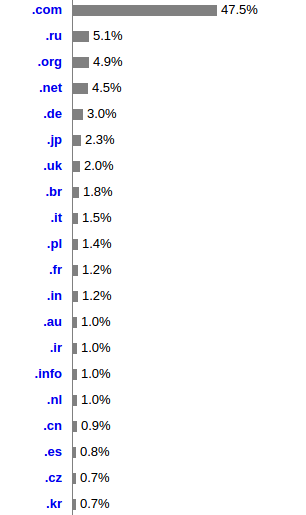
\includegraphics[scale=1]{image/TLD_all}\label{TLD_all}
		\caption{Popularność TLD w internecie (dostęp na dzień 15. maja 2017), źródło:  \cite{TLD_popularity}}
	\end{figure}
\end{center}  

\section{Analiza AS}
Podstawową informacją, którą uzyskać można wykorzystując pobrane dane z transferów AXFR jest przynależność otrzymanych adresów IP do konkretnych grup autonomicznych. Grupy te określają przynależność do sieci, które zarządzane są przed tego samego operatora sieciowego, a wykorzystuje się je głównie w protokołach routingu. Informacje związane z systemami autonomicznymi można, w głównej mierze, zanleźć w RFC1930\cite{RFC1930}.

Wartym uwagi jest fakt, że 

